\section*{Supplementary Material}

\subsection*{A. Additional Classification Ablation Figures}

\begin{figure}[H]
    \centering
    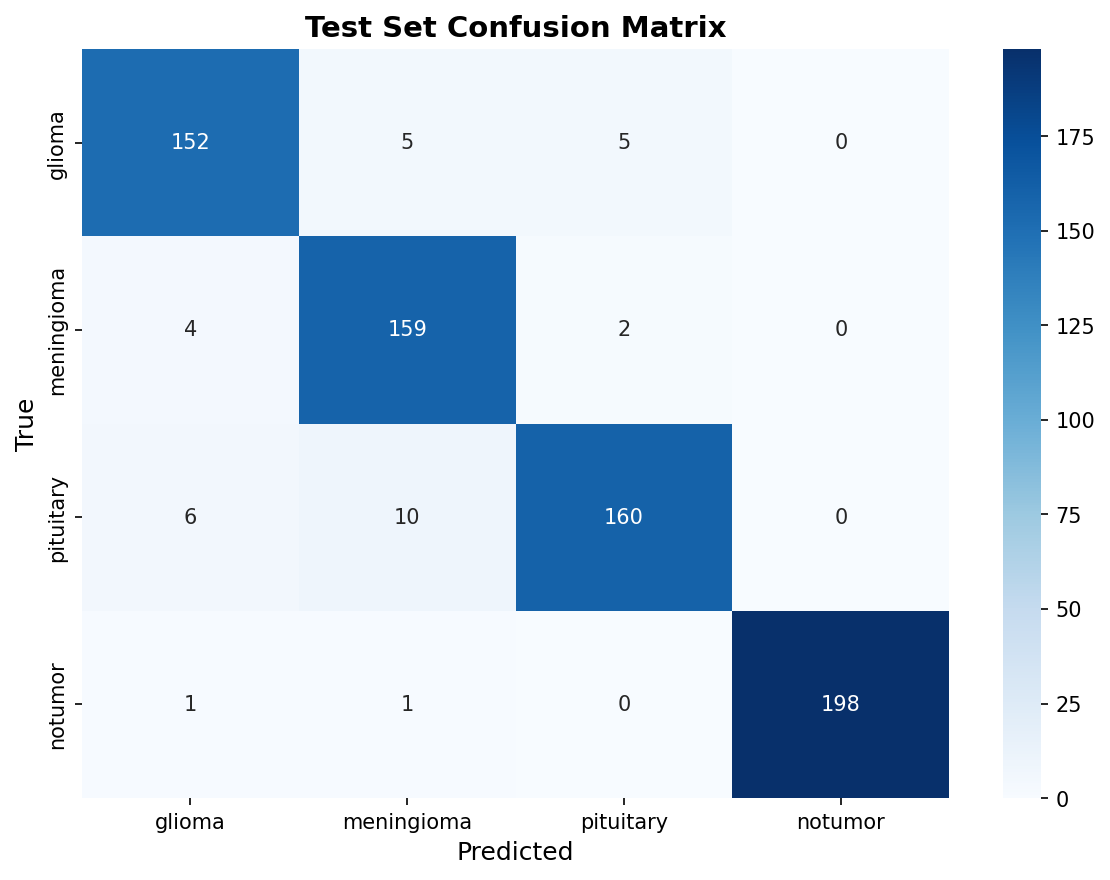
\includegraphics[width=0.5\textwidth]{figures/confusion_matrix_resunet_single.png}
    \caption{Confusion matrix for the cropped-only ResNet50 classifier.}
    \label{fig:supp_cm_resunet_single}
\end{figure}

\begin{figure}[H]
    \centering
    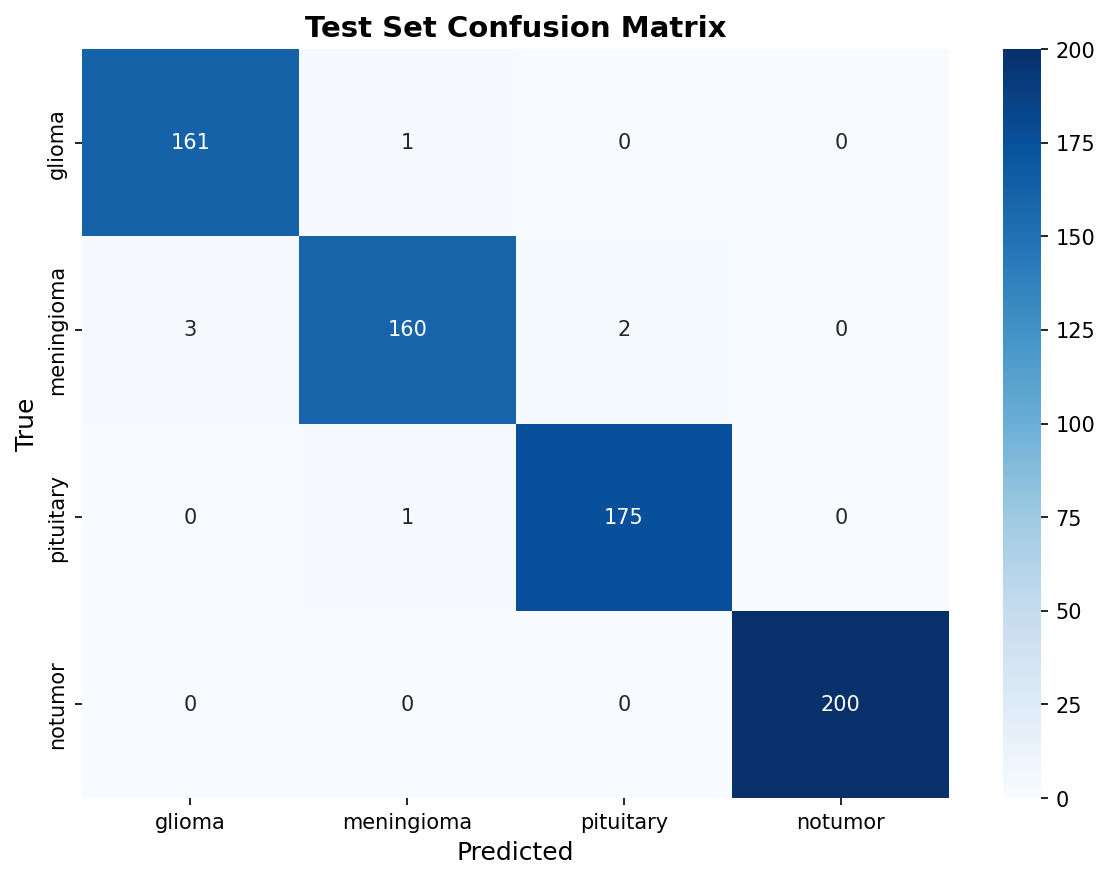
\includegraphics[width=0.5\textwidth]{figures/confusion_matrix_resunet_dual.png}
    \caption{Confusion matrix for the dual-input ResNet50 classifier.}
    \label{fig:supp_cm_resunet_dual}
\end{figure}

\begin{figure}[H]
    \centering
    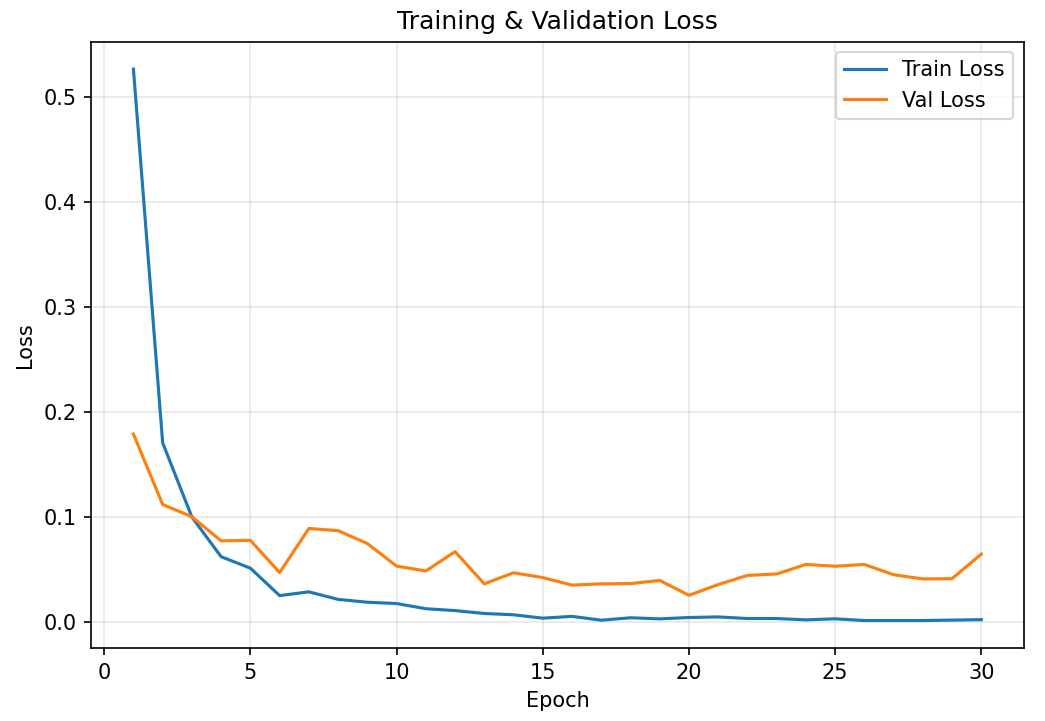
\includegraphics[width=0.7\textwidth]{figures/training_curves_resunet_dual.png}
    \caption{Training and validation curves for the dual-input ResNet50 classifier.}
    \label{fig:supp_dual_training_curves}
\end{figure}

\begin{figure}[H]
    \centering
    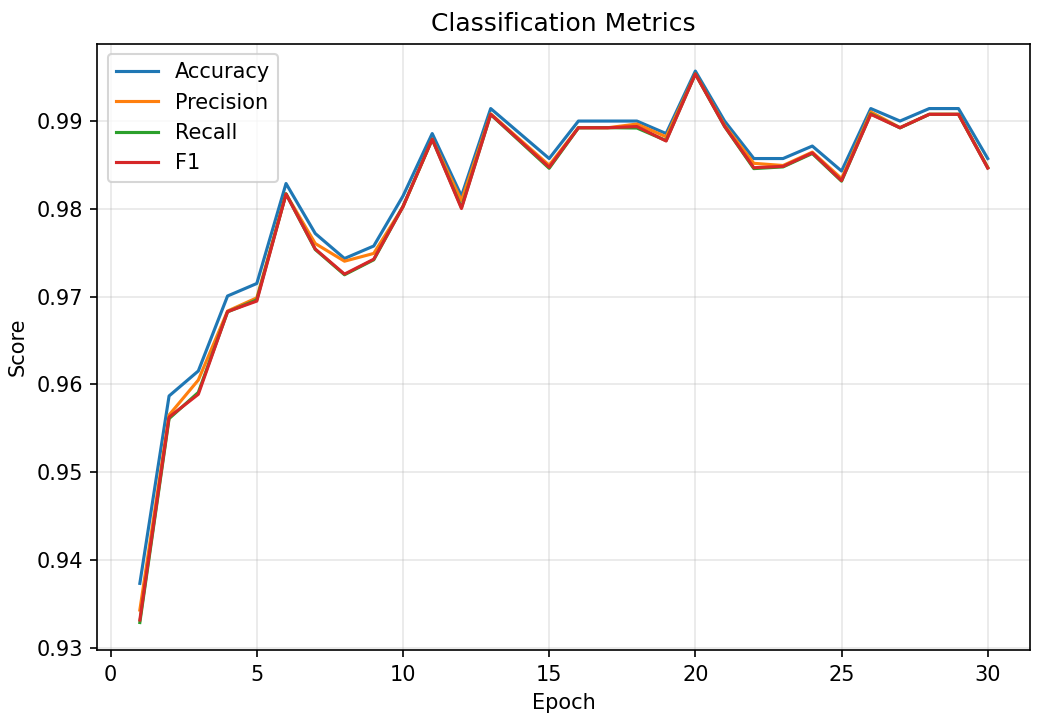
\includegraphics[width=0.7\textwidth]{figures/metric_curves_resunet_dual.png}
    \caption{Classification metric curves for the dual-input ResNet50 classifier.}
    \label{fig:supp_dual_metric_curves}
\end{figure}

\subsection*{B. Additional Qualitative Examples}
Figures~\ref{fig:supp_debug_notumor} and~\ref{fig:supp_debug_pituitary} show debugging examples from the final explainable pipeline. These examples include intermediate outputs such as the original MRI slice, available ground-truth or empty mask, predicted segmentation mask, Grad-CAM visualization, and generated VLM summary. They are useful for checking whether each stage of the pipeline behaves consistently during development.

\begin{figure}[H]
    \centering
    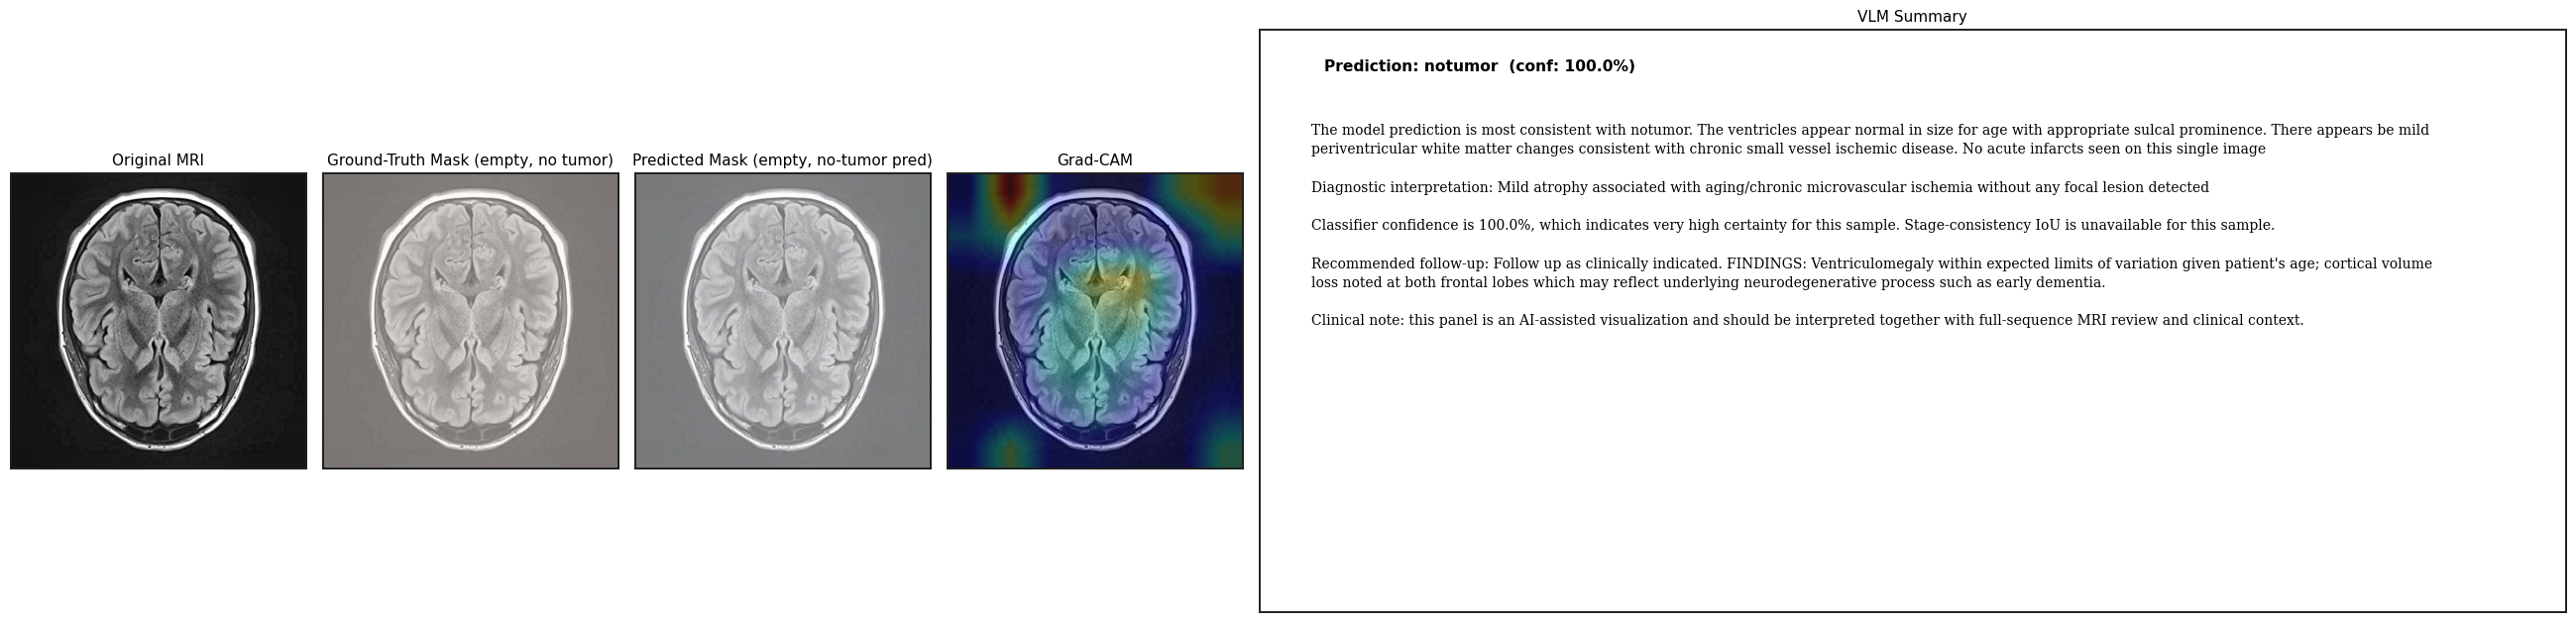
\includegraphics[width=1\textwidth]{figures/result4.png}
    \caption{Debugging example for a no-tumor case.}
    \label{fig:supp_debug_notumor}
\end{figure}

\begin{figure}[H]
    \centering
    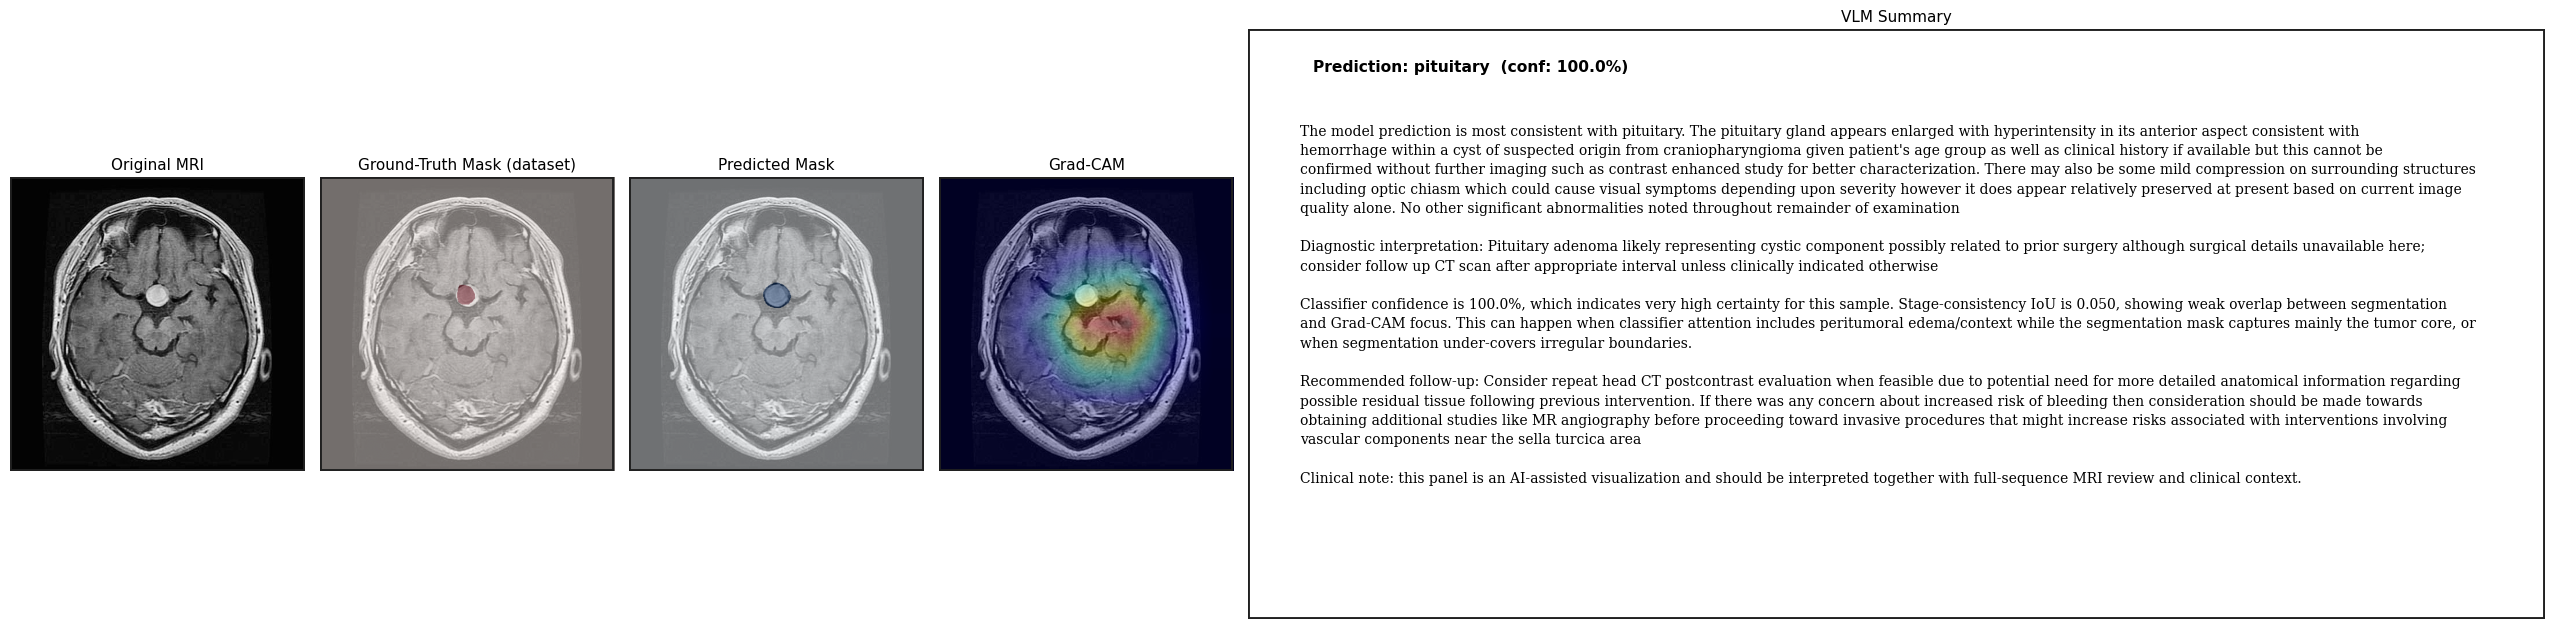
\includegraphics[width=1\textwidth]{figures/result3.png}
    \caption{Debugging example for a pituitary tumor case.}
    \label{fig:supp_debug_pituitary}
\end{figure}

Figures~\ref{fig:supp_real_notumor}, \ref{fig:supp_real_pituitary}, and~\ref{fig:supp_real_glioma} show more realistic inference examples where the ground-truth mask is not shown. These examples better reflect the expected deployment setting, where the system receives only an input MRI image and produces a predicted mask, Grad-CAM visualization, class prediction, and generated summary.

\begin{figure}[H]
    \centering
    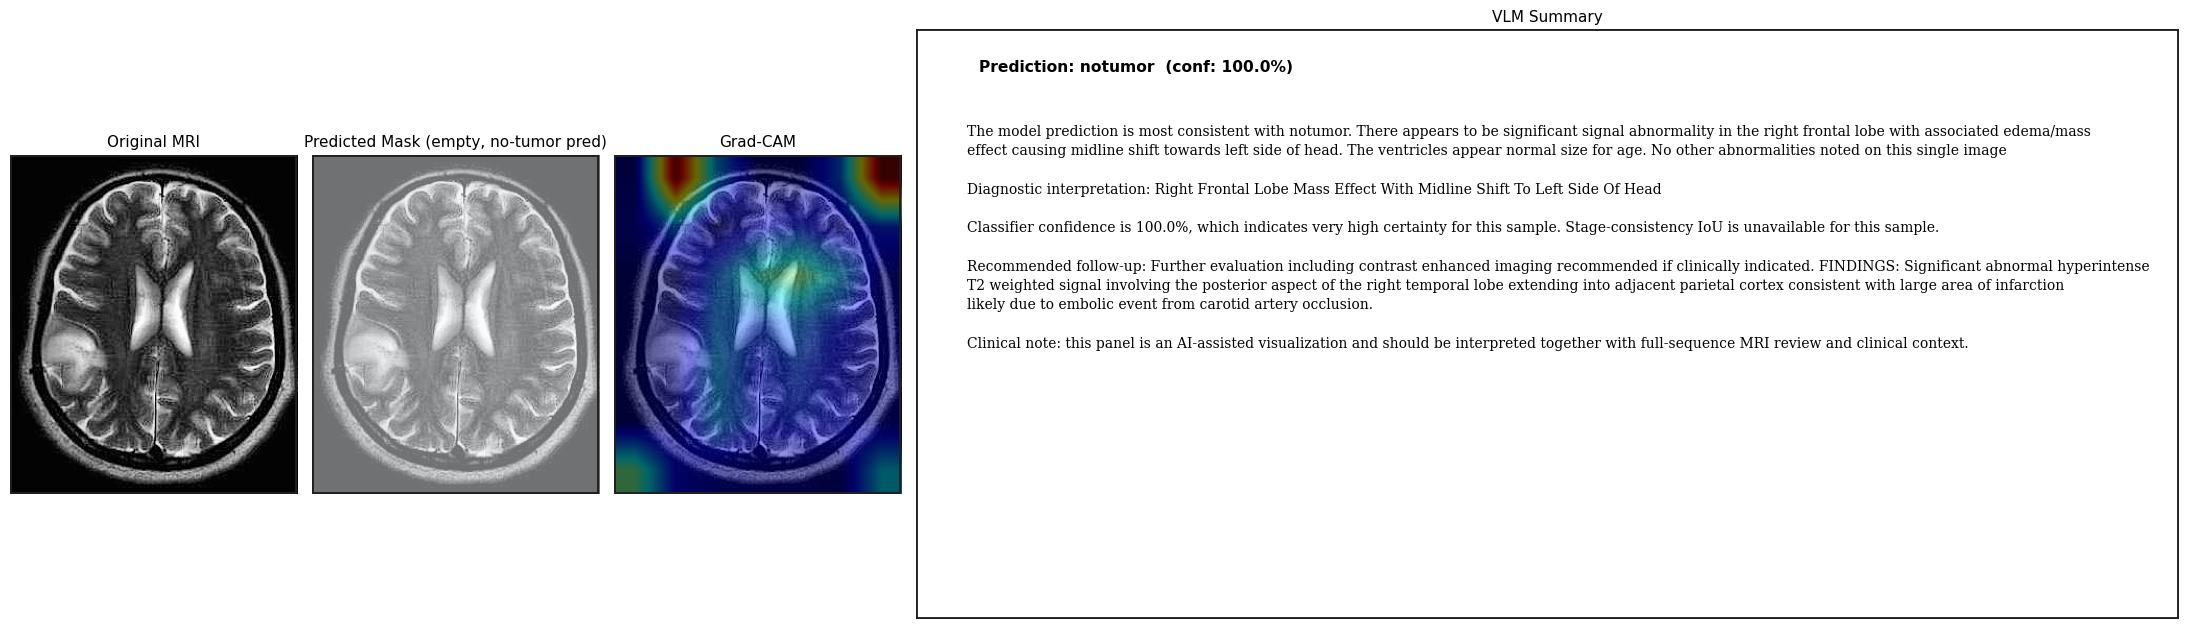
\includegraphics[width=1\textwidth]{figures/real_result2.png}
    \caption{Realistic inference example for a no-tumor case, without ground-truth mask shown.}
    \label{fig:supp_real_notumor}
\end{figure}

\begin{figure}[H]
    \centering
    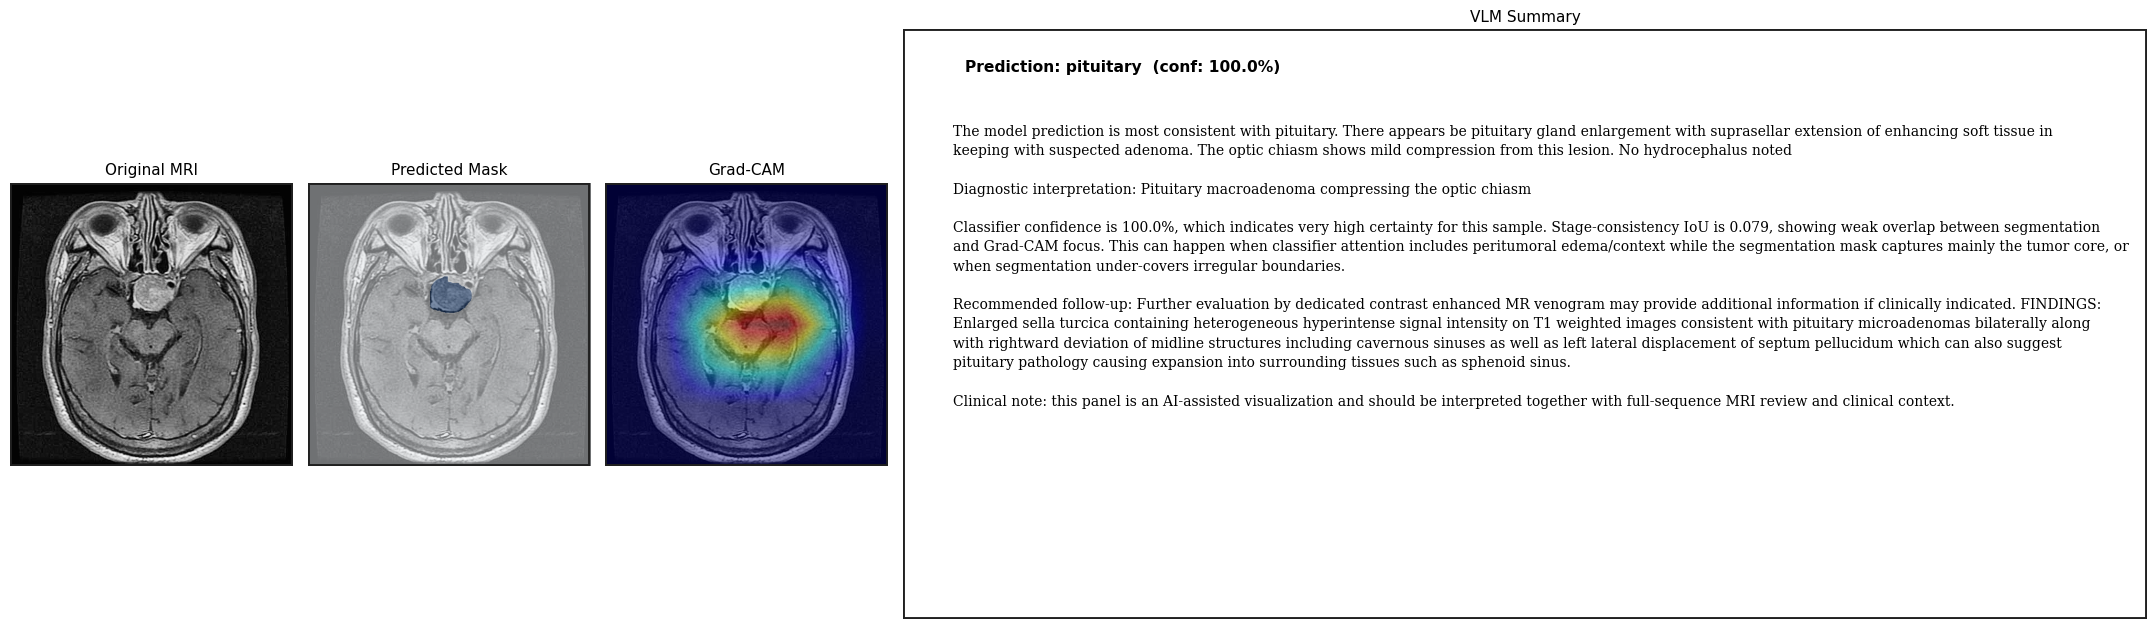
\includegraphics[width=1\textwidth]{figures/real_result1.png}
    \caption{Realistic inference example for a pituitary tumor case, without ground-truth mask shown.}
    \label{fig:supp_real_pituitary}
\end{figure}

\begin{figure}[H]
    \centering
    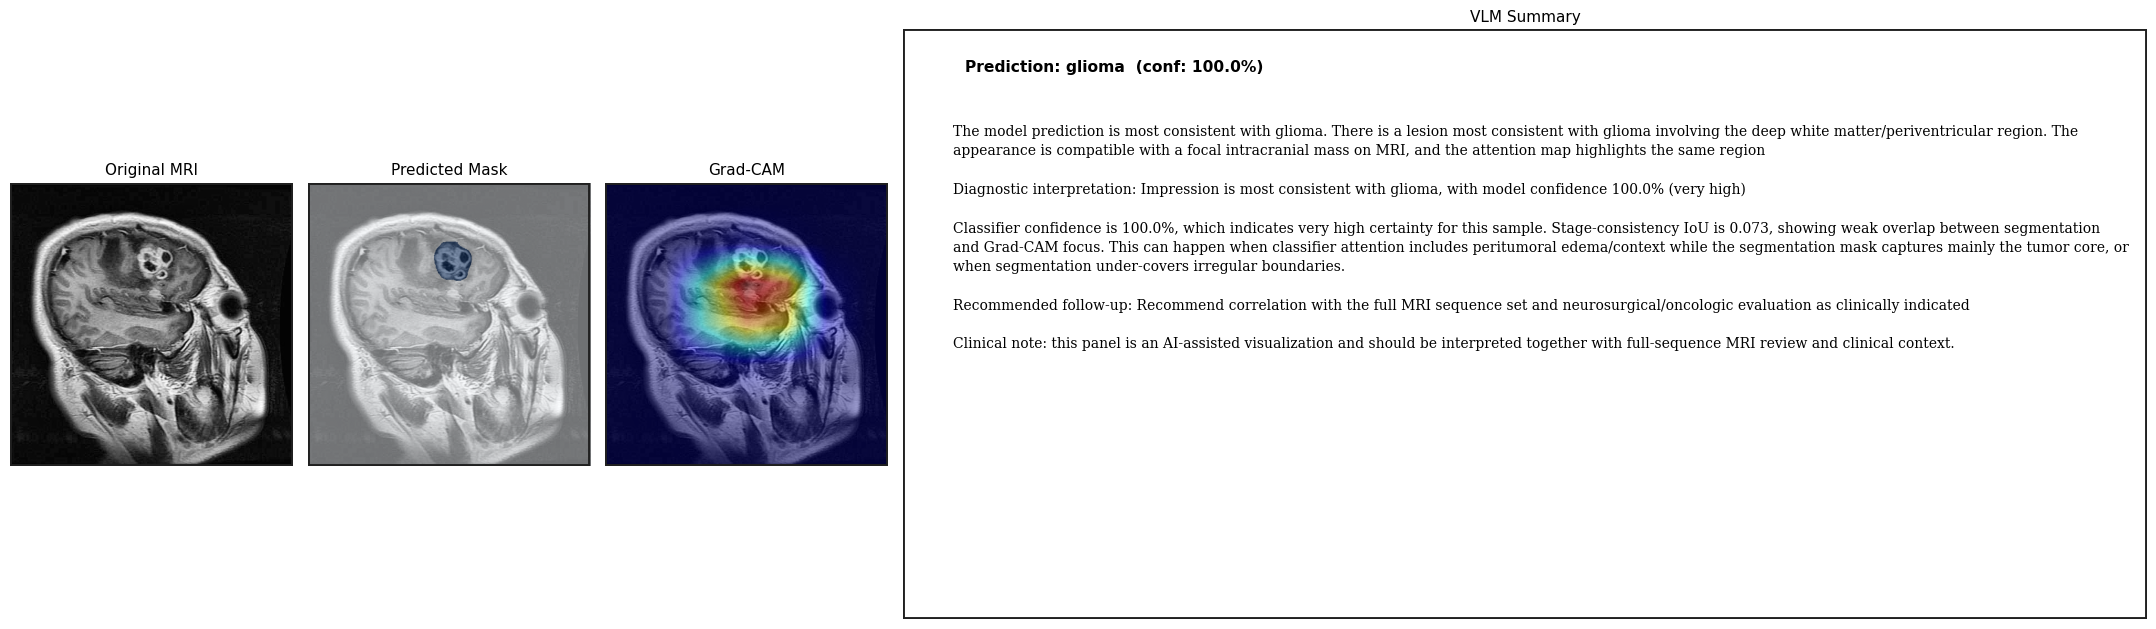
\includegraphics[width=1\textwidth]{figures/real_result3.png}
    \caption{Realistic inference example for a glioma case, without ground-truth mask shown.}
    \label{fig:supp_real_glioma}
\end{figure}

The VLM summary module is prompted in a zero-shot instruction format. The prompt conditions the model on the predicted class, confidence score, and Grad-CAM focus region, and asks it to produce a structured summary. If the generated output is malformed or inconsistent with the classifier prediction, the system falls back to a deterministic class-conditioned template. This fallback helps keep the generated explanation aligned with the model prediction.

